\section{Analysis of the Problem}
\subsection{Clarification}
Based on the ten smart growth principles in `The Smart Growth Network'\cite{pdf:smart-growth}, a  smart growth metric is to be set up which can well measure how successfully a city develops.
With two mid-sized cities on two different continents selected, the problem including the following requirements can be solved:

\subsection{Requirement}
\begin{enumerate}
  \item Using the metric above, judge whether the current growth plan of each city obeys the `smart growth principles', and measure how successfully each city grows.
  \item Based on the geography, economic opportunities and prospective, work out a growth plan for each city under the smart metric, and sequence every factor in the order of potential.
  \item Revise the growth plan in \textbf{2}, given that the population changed by 50\% till 2050.
\end{enumerate}

%-------------------------------------%
%-------------------------------------%
%-------------------------------------%

\section{The two mid-sized cities}
\subsection{Gernal information}
We choose \textbf{Nottingham} in Great British and \textbf{Barrie} in Canada as our target cities.
To simplify the functional distribution, we divide the two cities into square units (300m $\times$ 300m).
With the help of Google map and OpenStreetMap, the following data is collected:
\begin{itemize}
  \item Functional type of the block
  \item Development level (between 1 and 3)
  \item Bus stop number (or other public transport station)
\end{itemize}
To put it simple, we have the following figure \ref{fig:two-cities} showing the distribution.
\begin{figure}[htbp]
  \label{fig:two-cities}
  \centering
  \subfigure[Barrie development]{
    \label{fig:subfigure:barrie-development}
    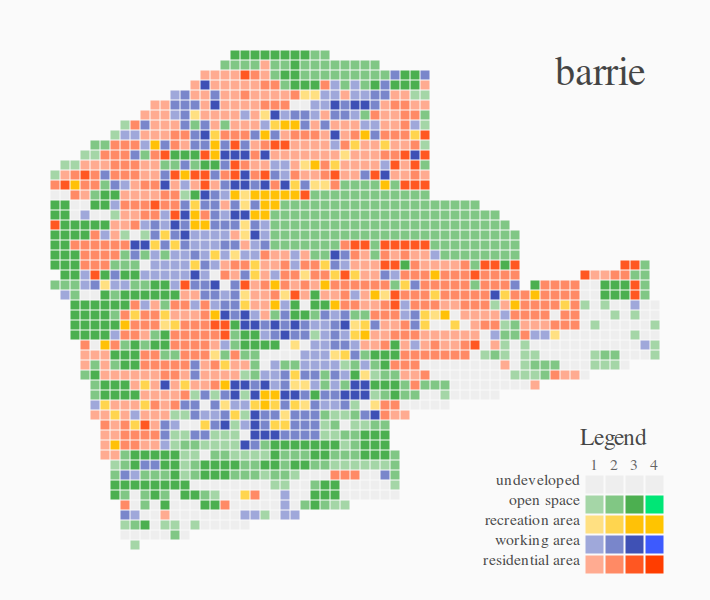
\includegraphics[width=6cm]{pic/barrie-development.png}
  }
  \subfigure[Barrie bus station]{
    \label{fig:subfigure:barrie-bus}
    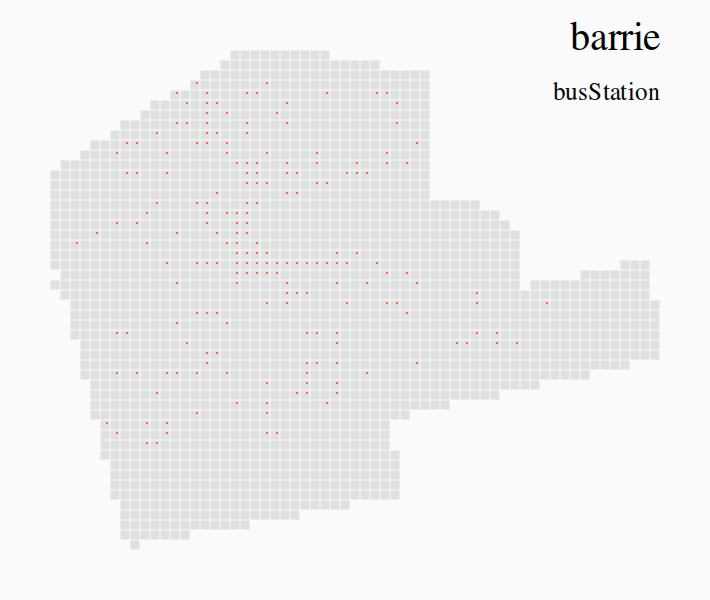
\includegraphics[width=6cm]{pic/barrie-busStation.png}
  }
  \subfigure[Nottingham development]{
    \label{fig:subfigure:nottingham-development}
    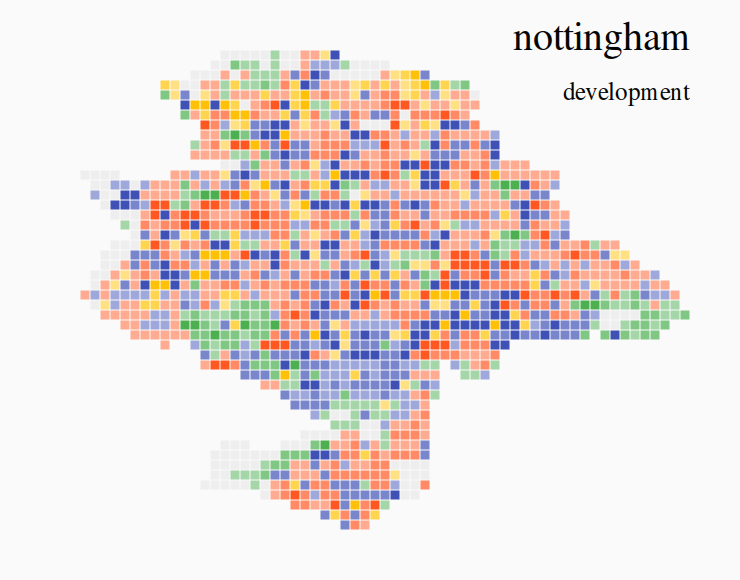
\includegraphics[width=6cm]{pic/nottingham-development.png}
  }
  \subfigure[Nottingham bus station]{
    \label{fig:subfigure:nottingham-bus}
    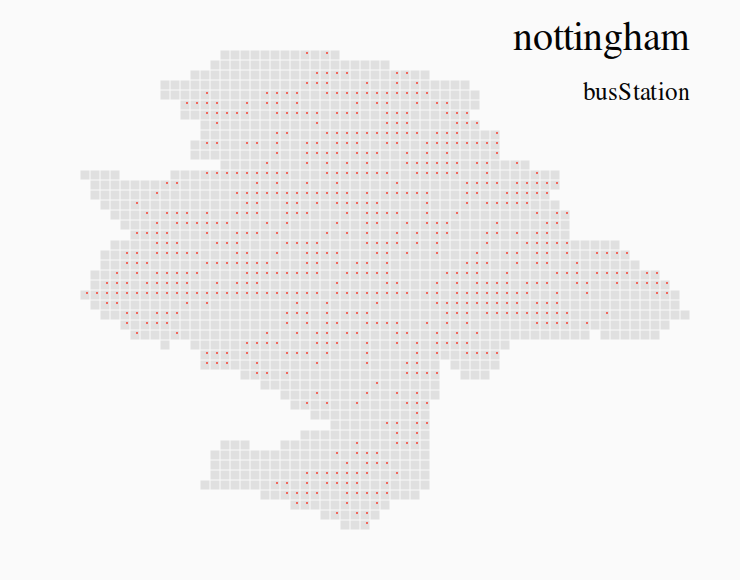
\includegraphics[width=6cm]{pic/nottingham-busStation.png}
  }
  \caption{}
\end{figure}

\subsection{Analysis of Nottingham}
\begin{table}
  \begin{tabular}{c|cccc}
    \hline
    Type & residential area & working area & recreation area & open space \\
    \hline
    Accounting for & 49.30\% & 32.07\% & 10.25\% & 13.96\% \\
    \hline
    Average level & 1.59 & 1.96 & 1.85 & 1.53 \\
    Average level*\footnote{(under government's plan)} & 1.66 & 2.28 & 2.05 & 1.53 \\
    \hline
  \end{tabular}
  \caption{Notthingham Distribution Data\footfullcite{pdf:the-nottingham-growth-plan}}
  \label{tab:nottingham-data}
\end{table}

As is shown in figure \ref{fig:subfigure:nottingham-development} \ref{fig:subfigure:nottingham-bus} and in table \ref{tab:nottingham-data}, the urban area of Nottingham city mainly consists of residential area, while open space accounts little.
It is worth noticing that working and recreational area has a relatively high development level, which is closely related to Nottingham's paying attention to technology, retail trade and advanced education.
However, it means that residential area has a lower development comparing to working area, indicating that the government's focus has long been on economic growth rather than people's happiness.
\\
\begin{table}
  \begin{tabular}{c|cccc|c}
    \hline
    Item & mix land use & beauty & residential choice & transport convenience & average \\
    \hline
    Score & 70.60 & 72.20 & 86.91 & 93.41 & 80.78 \\
    Score*\footnote{(under government's plan)} & 75.14 & 73.33 & 84.51 & 92.30 & 81.32 \\
    \hline
  \end{tabular}
  \caption{Notthingham Score under Smart Growth Metric}
  \label{tab:nottingham-score}
\end{table}
Combining data from table \ref{tab:nottingham-score} and distribution in figure \ref{fig:subfigure:nottingham-development} \ref{fig:subfigure:nottingham-bus}, we can find that working area contentrates in the middle part of the city's downtown, while residential and recreation area scatters around the downtown, which leads to a decrease in the score of mix land use.
As for the low performance in beauty, it seems contradictory to the temperate maritime climate, which is very suitable for plants to grow.
Nevertheless, if considering that Nottingham has a far more prosperous economy than the rest of Britain\footfullcite{wiki:nottingham-gdp}, it is not surprising that Notthingham, known as `a Technology City', inevitably sacrifices open space to give way to economic and technology development.
The low beauty score is against Principle 6, which emphasizes `critical environmental areas';
the convenient transport and diverse choices in residential area matches Principle 3 \& Principle 8.
\\
\begin{figure}[htb]
  \label{fig:nottingham-patch-diff}
  \centering
  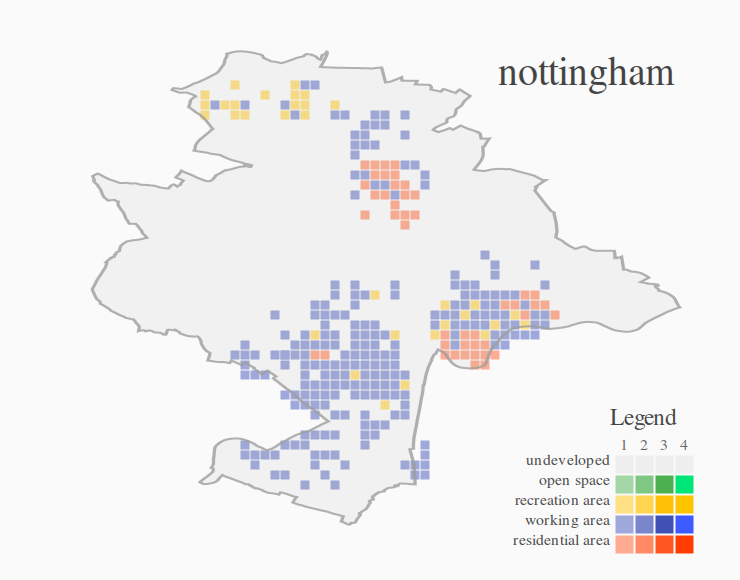
\includegraphics[width=6cm]{pic/nottingham-patch-diff-development.png}
  \caption{Nottingham development according to the government's plan}
\end{figure}
According to the government's growth plan and our smart growth metric, the city has some improvements, which is shown in figure \ref{fig:nottingham-patch-diff}.
It can be easily found that the following areas have a greater priority in the government's plan:
\begin{itemize}
  \item working area in downtown
  \item railway station neighbourhood
  \item northern residential and recreation area
\end{itemize}
To put it simple, the government still pays great attention to working area.
\\
As for the updated score under the government's plan in table \ref{tab:nottingham-data} and table \ref{tab:nottingham-score}, the residential choice score decreases due to the continuing ignorance of people's housing quality.
On the other hand, there is improvement in mix land use, for the sake of the development in the two area outside downtown.
\\
It is worth pointing out that, the growth plan we found doesn't refer to any development in open land; the file heavily depicts the techinal improvement for the city's landmarks - Boots and Biocity.
So it can be inferred that the government decides to further enhance the city's dominant industry.
The decision may meet its growth need to some extent, but it is still far from `Smart Growth Principle'.

\subsection{Analysis of Barrie}
\begin{table}
  \begin{tabular}{c|cccc}
    \hline
    Type & residential area & working area & recreation area & open space \\
    \hline
    Accounting for & 35.3\% & 20.97\% & 15.47\% & 36.30\% \\
    \hline
    Average level & 1.66 & 1.78 & 2.08 & 2.16 \\
    \hline
  \end{tabular}
  \caption{Barrie Distribution Data}
  \label{tab:barrie-data}
\end{table}

As is shown in figure \ref{fig:subfigure:barrie-development} \ref{fig:subfigure:barrie-bus} and in table \ref{tab:barrie-data}, working and recreation area has a rather small portion, while recreation area and open space develops much better than the rest.
The city of Barrie can be divided into three S-shape stripe zones: the left part is mostly residential, the middle part commercial, the right part mixing residents and recreation.
The high development of recreation area should owe to various winter-sport stadiums in the right zone, which is also a feature of city Barrie.
The heavy forest and large water area around the borderline of Barrie adds to the natural environment of the city's beauty; however, the heavy occupancy of land also forms an obstacle to the commercial development.
Comparing to Nottingham's terrian (see figure \ref{fig:subfigure:nottingham-development}), Barrie has a lower density of working area at the borderline, which may interfere with commercial communication.
\\
\begin{table}
  \begin{tabular}{c|cccc|c}
    \hline
    Item & mix land use & beauty & residential choice & transport convenience & average \\
    \hline
    Score & 54.24 & 92.11 & 64.06 & 50.67 & 65.27 \\
    Score*\footnote{(under government's plan)} & 57.93 & 92.50 & 62.73 & 57.70 & 67.72\\
    \hline
  \end{tabular}
  \caption{Barrie Score under Smart Growth Metric}
  \label{tab:barrie-score}
\end{table}
In table \ref{tab:barrie-score}, the first three scores reflects that the three `S-stipe zones' largely interrupts Barrie's adapting to `Principle 1'(mix land use) and housing choice in `Principle 3'.
It's worth mentioning that roads in Barrie are a lot wider (and the distribution is more discrete than in Nottingham), so people tenf to drive instead of taking a bus, which is contrary to diverse transport choices in `Principle 8'.
\\
We looked up for the plan of Barrie government \cite{pdf:barrie-downtown-plan} \cite{pdf:barrie-waterfront} \cite{pdf:barrie-official-plan} \cite{pdf:barrie-industrial-mapping} and arrange out the following improvements, shown in figure \ref{fig:barrie-patch-diff}.
\begin{figure}[htb]
  \label{fig:barrie-patch-diff}
  \centering
  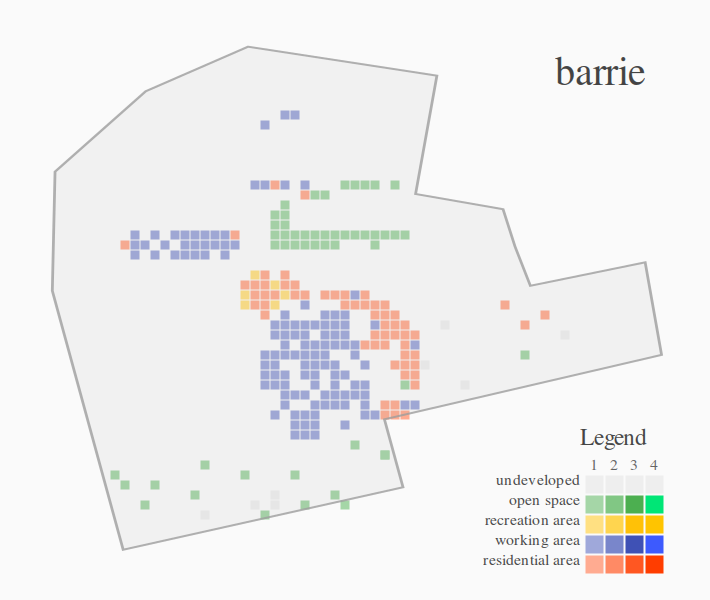
\includegraphics[width=6cm]{pic/barrie-patch-diff-development.png}
  \caption{Barrie development according to the government's plan}
\end{figure}
The government seems to have realized their ignorance in commercial, so the improvements concertrated in the mid S-stripe zone, the right stripe zone and at the same time improve the lake area.
It is obvious that the government still pays great attention to economic development, since 55.35\% efforts are made to working area.
The score under the government's plan is shown in table \ref{tab:barrie-score}.
\\
The government of Barrie seems to take a very different approach from that of Nottingham; it emphasizes its weak points rather than becoming a tourism city.
However, the S-shape stripe zones still largely interfere with the diverse development.
It is hard to make a big change in the city's functional distribution just in a short time of 10 years.

%-------------------------------------%
%-------------------------------------%
%-------------------------------------%

\printbibliography

%-------------------------------------%
%-------------------------------------%
%-------------------------------------%
